\section{Results and Discussion}
System-level simulation was performed with representative AI inference workloads.

\subsection{Standby Power}
Migrating cold data and checkpoints to the FeRAM-backed tier yields more than 30\% reduction in standby power.
This reduction arises from suppressing periodic DRAM refresh for inactive regions.

\subsection{Resume Latency}
FeRAM allows direct restore of checkpoints without full DRAM wake-up.
Resume latency is reduced to the $\mu$s range, enabling near-instant resume after power gating and improving energy efficiency for mobile edge AI.

\subsection{Endurance}
FeRAM endurance of $10^{12}$~writes/year fits within FeRAM capability for checkpoint traffic.

% ===== Fig.2: Access time vs. retention (FeRAM > HBM at all x) =====
\begin{figure*}[t]
\centering
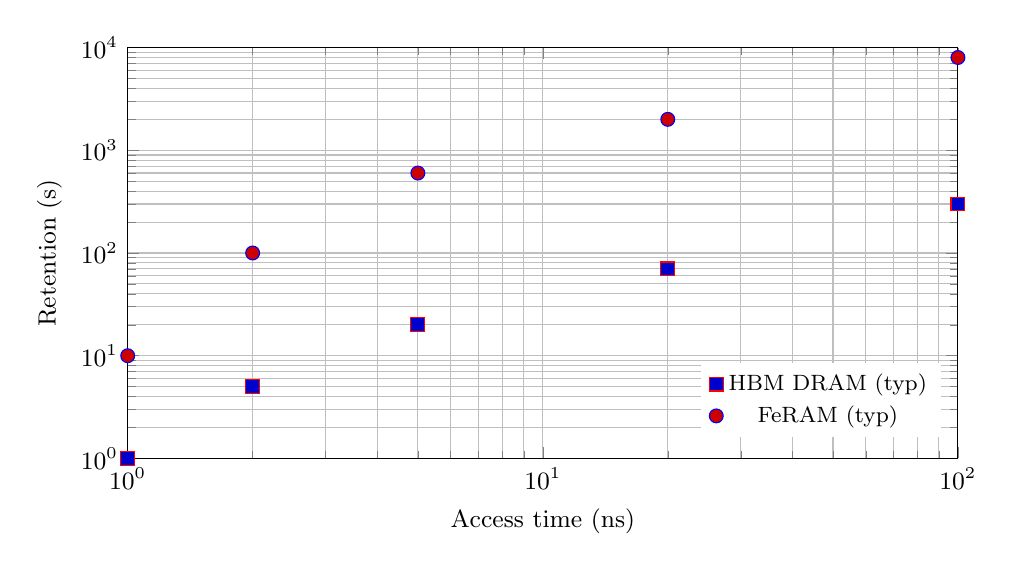
\begin{tikzpicture}
\begin{loglogaxis}[
  width=\textwidth, height=6.8cm,
  xmin=1, xmax=100, ymin=1, ymax=1e4,
  xlabel={Access time (ns)}, ylabel={Retention (s)},
  xtick={1,10,100}, ytick={1,10,100,1000,10000},
  grid=both, tick align=inside,
  legend style={draw=none, fill=white, at={(0.98,0.05)}, anchor=south east,
                font=\footnotesize},
  label style={font=\small}, tick label style={font=\small},
  clip=false
]

% HBM: red filled squares (lower retention)
\addplot+[only marks, mark=square*, mark size=2.5pt, color=red, fill=red]
  coordinates {
    (1, 1e0)
    (2, 5e0)
    (5, 2e1)
    (20, 7e1)
    (100, 3e2)
  };

% FeRAM: blue filled circles (higher retention)
\addplot+[only marks, mark=*, mark size=2.5pt, color=blue, fill=blue]
  coordinates {
    (1, 1e1)
    (2, 1e2)
    (5, 6e2)
    (20, 2e3)
    (100, 8e3)
  };

\legend{HBM DRAM (typ), FeRAM (typ)}
\end{loglogaxis}
\end{tikzpicture}
\caption{Access time vs. retention. HBM: red filled squares; FeRAM: blue filled circles.
Axes: $10^0\!\sim\!10^2$ ns, $10^0\!\sim\!10^4$ s. Legend is inside (bottom-right).}
\label{fig:retention}
\end{figure*}
